%Results
\section{Descriptive statistics}
Before the experiment, the seeds were weighted in groups of ten, to see if there was a baseline difference between certain genotypes. Table \ref{tab:germination_percentage}, in the previous section, displays the measured weights.
After the completion of the experiment, the outliers were identified, and each plant was attributed a specific weight, following the protocol described in material and methods section. Those weights were used to compute the weighted mean and weighted standard deviation of the fresh and dry weight of the root system and the leaf system, as well as the area of the root system, for each plant. Dotplots representing those descritptive statistics as well as the data point are presented in figure \ref{fig:dotplot_all_variables}. The numerical values of these results are presented in table \ref{tab:summary_table_all_variables}, in appendix \ref{appendix:mean_std_table}.\\

Even though no clear conclusions can be made from these figures, we can see large variation of mean values between genotypes. Also, for some genotypes, the difference between tanks seem significant (e.g. genotype 15) while it's clearly not the case for some other (e.g. genotype 7). This implies that the tank and genotypes effects are significant. Overall the values of dry weights seem to have less variations than the fresh weights.

\begin{figure}
\centering
	\begin{subfigure}[t]{\textwidth}
		\centering
		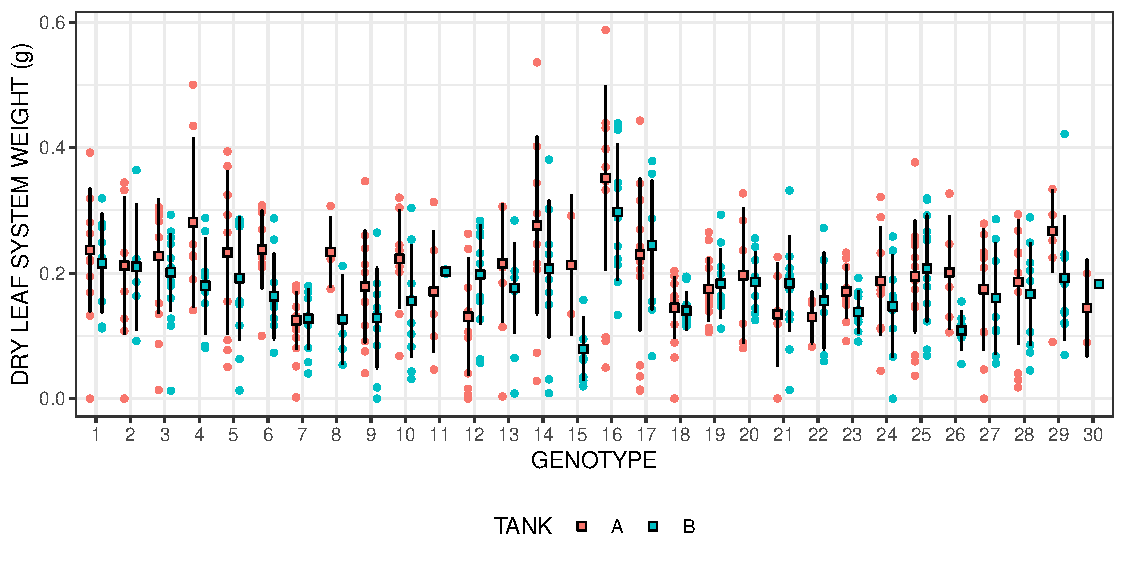
\includegraphics[width = \textwidth]{../../Figures/DRY_LS_summary_plot.pdf}
		\caption{Dry leaf weight ($DRY\_LS$)}
	\end{subfigure}

	\begin{subfigure}[t]{\textwidth}
		\centering
		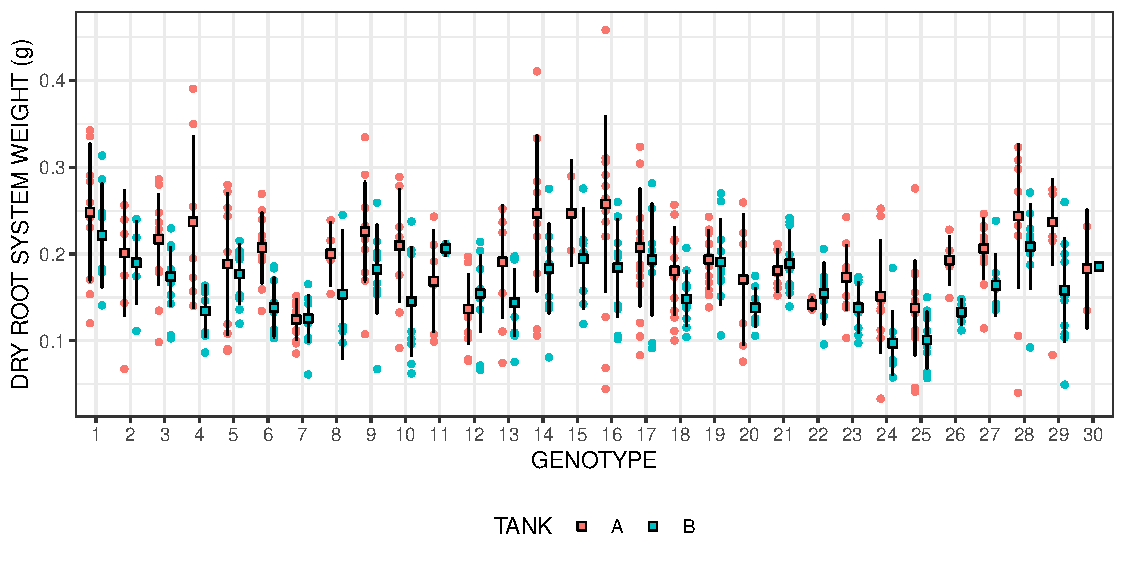
\includegraphics[width = \textwidth]{../../Figures/DRY_RS_summary_plot.pdf}
		\caption{Dry root weight ($DRY\_RS$)}
	\end{subfigure}
	\caption{Dotplot displaying mean weight (\protect\emptysquare) and associated standard deviation (\protect\blackline), grouped by tanks for each variable.}
\end{figure}
\begin{figure}\ContinuedFloat
	\begin{subfigure}[t]{\textwidth}
		\centering
		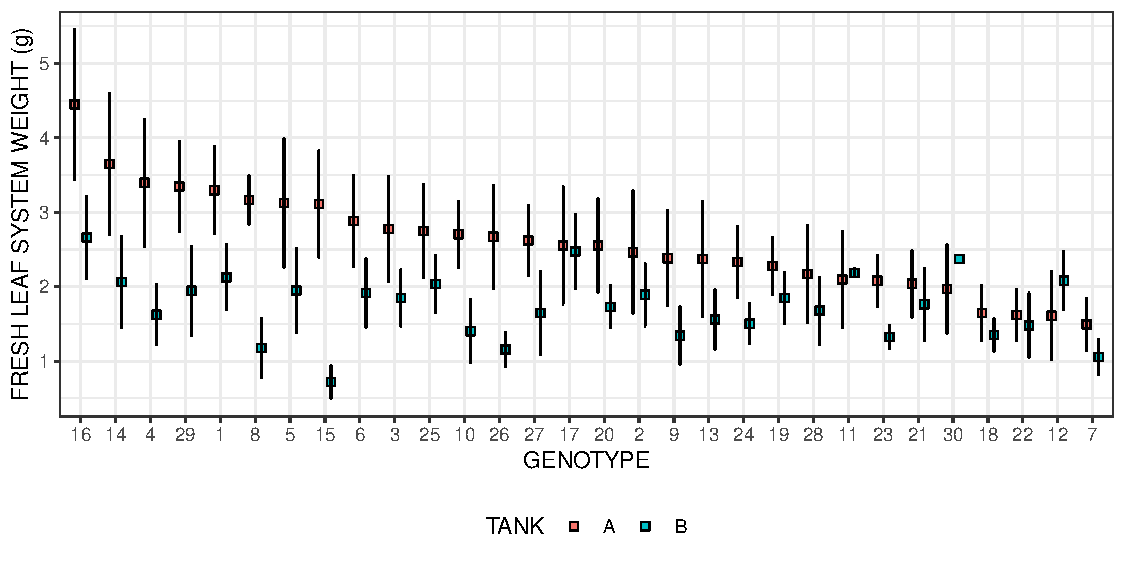
\includegraphics[width = \textwidth]{../../Figures/FRESH_LS_summary_plot.pdf}
		\caption{Fresh leaf weight ($FRESH\_LS$)}
	\end{subfigure}

	\begin{subfigure}[t]{\textwidth}
		\centering
		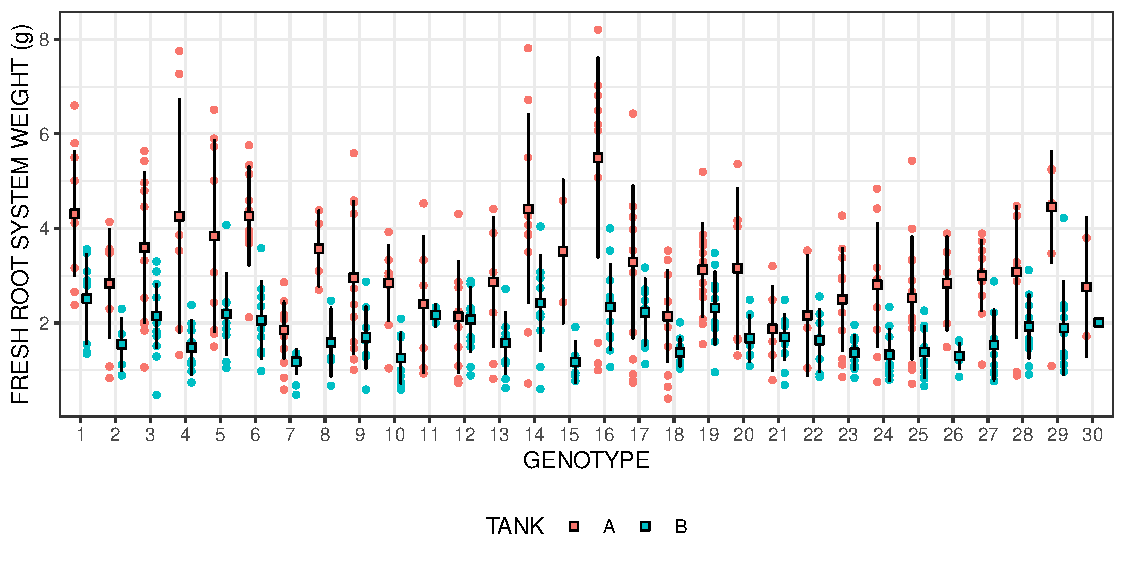
\includegraphics[width = \textwidth]{../../Figures/FRESH_RS_summary_plot.pdf}
		\caption{Fresh root weight ($FRESH\_RS$)}
	\end{subfigure}
	\caption{Dotplot displaying mean weight (\protect\emptysquare) and associated standard deviation (\protect\blackline), grouped by tanks for each variable.}
	\label{fig:dotplot_all_variables}
\end{figure}

\section{SpATS analysis}


\section{ARxAR model analysis}
\section{Model comparison}
\subsection{Performances}
\subsection{Parametrization}
\subsection{Modelling strategy}
